% Chapter 1

\chapter{Analysis} % Chapter title

\label{ch:analysis} % For referencing the chapter elsewhere, use \autoref{ch:architecture} 

%----------------------------------------------------------------------------------------



\section{Audience}

Throughout this report we have mentioned in detail the characteristics of the application: its requirements to function properly, the decisions that need to be made in order for it to produce reliable results and the problematic parts of it that require attention in order to avoid erroneous results. Taking all of the above into consideration, we have concluded on a group of people that not only will find this application useful, but will also know how to use it to its full extent and potential.\\
Surely, the product of our work is not meant to be operated by everyone, even though that would be quite desirable. There is a limit on which people can operate our product in an efficient manner and that fact comes from the various components that were needed in order to create such application. A lot of considerations that we have made are so in order to ensure that our application is available to the widest possible audience. Unfortunately, there are elements that for better or worse, limit that audience.
To begin with, we believe that the setup and interface of the application is as straightforward as possible. That ensure that it is easy to use and understand by anyone. As the user goes on in the application that changes. When we require the user to upload an image, then he/she needs to understand that the application performs at its fullest when provided with an elevation model that uses the WGS84 geographical reference system. That fact alone, requires some amount of knowledge in the fields of geography, surveying or cartography.\\

Another limiting factor is the actual input of the application. As presented above, the elevation model is the most important input the user has to provide. After the upload the user will then designate the source of the flood. As presented above, that approach requires great attention because an erroneous selection of the flood source can result in failure of the process. This entire process of designating the flood and making sure that the source point is within the extent of the raster requires a certain acquired experience with working with rasters.
Finally, another deciding factor that sets limitations on who can use this application is the hydrologic aspect of it. This aspect concerns the evolution of the flood event, its spread across the landscape as well as the management of the event. To be more specific, we believe that in order to use this tool at its maximum extent and produce reliable results and create efficient solutions, the user would probably need to have some experience with hydrology. That is because the tool uses a number of terms from that field in order to produce the results it does and understanding these terms and how they affect the results of the process is important to design viable solutions.


\section{Installation structure}

Now that the application has been implemented, it is relevant to analyze how the entire installation is structured on the server. As mentioned in the \autoref{ch:implementation} part, a variety of softare packages have been installed on the server, these being 

\begin{itemize}
\item PyWPS
\item Flask
\item Apache2
\item GRASS
\end{itemize}

\paragraph{Debugging:} When the server has been installed, it runs on it's own, and not much else has to be manipulated with from then on. When the process fails for some reason, it can be relevant to troubleshoot the problem by reading the error log. Both Apache and PyWPS have error logs that can provide information about the situation, which can help to fix the error. The logs for both of these critical components can be found in the directories shown on \autoref{fig:anal_struct}:\\

\begin{figure}[h]
\dirtree{%
.1 /.
.2 /var/.
.3 /www/.
.4 /html.
.5 /pywps/.
.6 pywps\.log.
.3 /log/.
.4 /apache2/.
.5 error\.log.
}
\caption{Location of the error logs.}
\label{fig:anal_struct}
\end{figure}

\paragraph{PyWPS installation:}Accessing the PyWPS installation: When wanting to change, or modify, some of the functionality of PyWPS, it is necessary to access the server and perform the changes here. The setup is displayed in \autoref{fig:pywpsinstall}. 

\begin{figure}[h]
\dirtree{%
.1 /.
.2 /var/.
.3 /www/.
.4 /html.
.5 /pywps/.
.6 pywps\.log.
.6 pywps.cfg.
.6 /processes/.
.7 \_\_init\_\_.py.
.7 process1\.py.
}
\cation{Structure of the PyWPS installation.}
\label{fig:pywpsinstall}
\end{figure}

When adding or removing processes, it has to be done in the processes folder. The process is added (or removed) from the drive, and the \_\_init\_\_.py file is modified to reflect the change that has occurred in the drive.

A variety of serverside settings can be managed from the pywps.cfg file, for instance the maximum allowed filesize of a DEM used as input, or the location of PyWPS outputs.

\paragraph{Flask installation:}Flask is installed in the directories shown on \autoref{fig:flaskinstall}.\\

\begin{figure}[h]
\dirtree{%
.1 /.
.2 /var/.
.3 /www/.
.4 /html.
.5 /FlaskApp/.
.5 flaskapp\.wsgi.
.6 /FlaskApp/.
.7 /templates/.
.7 /images/.
.7 /static/.
.7 \_\_init\_\_.py.
}
\caption{Installation structure of Flask}
\label{fig:flaskinstall}
\end{figure}

It is within the \_\_init\_\_.py file that most changes mentioned in the Implementation section have been performed. The templates folder contains the templates used to display HTML. The static folder contains a variety of static content, such as the jQuery and CSS libraries. A functionality of Flask is that content on the server that isn't directly served by the user, isn't meant to be accessible. But if it is placed within the static folder, and the url to the content is known, it can be accessed from “outside”. The outputs of the PyWPS service are therefore directed to a subdirectory of the static folder, so that we can easily access the data through the website front-end.
The images folder is used to store the DEM the user uploads, and works with through the entire process.\\

\paragraph{GRASS Installation:}The GRASS installation is fairly simple (and the structure can be seen in \autoref{fig:grassinstall}), and after the initial setup is not touched, even when adding new functionalities. The grassdata folder normally contains the various locations and mapsets that are used by the user. In our case the folder only contains one LOCATION, projected to WGS84. This will be used by the PyWPS process to work with the data in question. 
The .grassrc6 folder contains some settings that are needed for GRASS to function properly.

\begin{figure}[h]
\dirtree{%
.1 /.
.2 /home/.
.3 /ubuntu/.
.4 \.grassrc6.
.4 /grassdata/.
.5 <LOCATION>.
.6 <MAPSET>.
}
\caption{Installation folder structure of GRASS}
\label{fig:grassinstall}
\end{figure}


\section{Architecture}
\begin{figure}[h!]
\centering
	{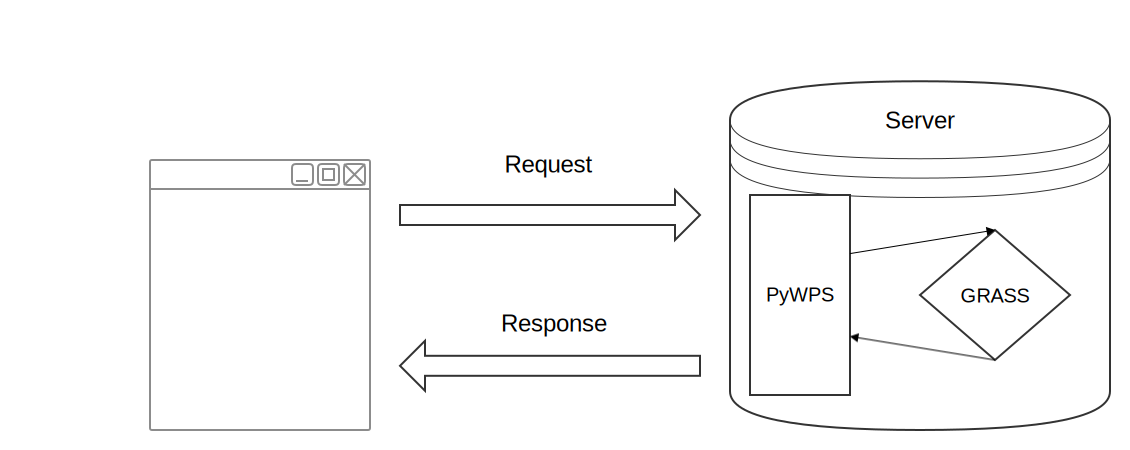
\includegraphics[width=\linewidth]{gfx/Analysis_Architecture/grass_pywps.png}}
\caption{The architecture of the software}
\label{fig:grass_archi}
\end{figure}


\section{User experience}
In this part of the report we will present  how our web service works for the point of view of the user. What we will do, is try to demonstrate as detailed as possible the actual results of the phases we described on the previous chapter. We will also include a step-by-step guideline on how the service should be used and what actions are necessary for the user to follow in order to get the best results possible out of this process. But before we go in depth of the structure of the website, we will take a look at the overview of the setup, as seen on \autoref{fig:analysis_1}

\begin{figure}[h!]
\centering
	{\includegraphics[height=0.33\textheight]{gfx/Analysis_Website/1.jpg}}
\caption{Overall workflow of the application}
\label{fig:analysis_1}
\end{figure}

We begin by presenting the first page the user will see when they visit our website \autoref{fig:analysis_frontpage}. The url that leads to the homepage of the application is http://52.17.144.192/. The first page is then displayed that provides information about the website such as its name and a basic description of what services it offers (\autoref{fig:analysis_2}

\begin{figure}[p]
  \myfloatalign
  \subfloat[Banner.]
  {\label{fig:analysis_2}  
  {\includegraphics[width=\linewidth]{gfx/Analysis_Website/2.png}}} \quad
  \subfloat[Banner]
  {\label{fig:analysis_3}  
  {\includegraphics[width=0.45\linewidth]{gfx/Analysis_Website/3.png}}} \quad
  \subfloat[Middle.]
  {\label{fig:analysis_4}%
   \includegraphics[width=0.45\linewidth]{gfx/Analysis_Website/4.png}} \\
 \caption{Frontpage of the web application, tentatively dubbed \textit{flooding}.}
 \label{fig:analysis_frontpage}
\end{figure}

Lower on the same page, we provide the user with detailed information about the application. The reason we have created it, who can use it and its most important advantages and features \autoref{fig:analysis_3}

On the final part of the page, we provide the user with small examples of the programming languages, frameworks and other tools we used on order to create this service 
\autoref{fig:analysis_4}

In order to proceed with the actual simulation the option FLOOD on the first part of the page has to be chosen. That will create a new tab on the browser that leads to the second part of the website (\autoref{fig:analysis_upload}). This part is a guided process of the flood simulation that follows. By clicking on the Commence flooding option, the initial part of the flood commences.

\begin{figure}[p]
  \myfloatalign
  \subfloat[Page describing the coming process.]
  {\label{fig:analysis_2}  
  {\includegraphics[width=\linewidth]{gfx/Analysis_Website/5.png}}} \quad
  \subfloat[Uploading a DEM.]
  {\label{fig:analysis_3}  
  {\includegraphics[width=\linewidth]{gfx/Analysis_Website/6.png}}} \quad
 \caption{Accessing the possibility of uploading a DEM.}
 \label{fig:analysis_upload}
\end{figure}

The process starts with requesting the user for the necessary input in order for the application to run (\autoref{fig:analysis_6}). As mentioned in previous parts of the report, that necessary input is an elevation model. 

Once the user chooses an elevation model from his local hard drive and then uploads it, the second step is initialized (\autoref{fig:analysis_7}). 


\begin{figure}[h!]
\centering
	{\includegraphics[width=\linewidth]{gfx/Analysis_Website/7.png}}
\caption{Step 2 display uploaded elevation model and insert point to designate origin of flood}
\label{fig:analysis_7}
\end{figure}

the application the user is called to provide it with the ocean. In other words, where he wants the flood to originate from. By simply clicking on the map, that point is created. 
Finally, the user then has to decide which type of process he/she wishes to perform. The simple flood option will instantly fill the elevation model with a predefined level of water and display the results on a map on the third step (\autoref{fig:analysis_8}).

\begin{figure}[t]
\centering
	{\includegraphics[width=\linewidth]{gfx/Analysis_Website/8.png}}
\caption{Results of the simple flood option}
\label{fig:analysis_8}
\end{figure}

\section{Limitations}
In this section, we will discuss the existing limitations the users might face while using our application. These limitations are either placed by us, to ensure that our application works at an optimal level or exist purely because of the features and the parts that consist it. Regardless of the origins of these limitations, we think that it is our responsibility to let the user know about them and notify them before using the application, so that we can save them time while using it.

\paragraph{Extensions and filename:} The first limitation we set is during the uploading of the input by the user. In an effort to apply some sort of control on what the user is capable of uploading to our server, we made sure that only certain file types are allowed for upload. The reason behind this specific action is that we do not want to allow any kind of file in our server. Mainly because we want to make sure that the memory of the server is reserved for files that are actually compatible with the application but also install a first wall of security against malicious intents. That being said, the user can only upload .tiff files. This file type check is performed in two steps. First, we declare the types that are allowed for upload.

\begin{lstlisting}
ALLOWED_EXTENSIONS = set(['tif'])
\end{lstlisting}

Then we create a function that checks the extension of a file-to-be uploaded and if it is included in the ALLOWED EXTENSIONS, basically a tiff file, it returns a true  value:

\begin{lstlisting}
def allowed_file(filename):
	return '.' in filename and \
			filename.rsplit('.',1)[1] in ALLOWED_EXTENSIONS
\end{lstlisting}

Finally, we set a condition that checks the result of the function mentioned above and if it is true, then it proceeds with uploading the file, otherwise it will reload the upload page without any results

\begin{lstlisting}
#check if the extension is allowed
if allowed_file(file.filename):
\end{lstlisting}

Having said that, the main reason we decided to use tiff as the only allowed extension the uploaded file can have is because tiff files contain necessary spatial information of the file. To be more precise, important information about the geographical reference system, the projection in use and the coordinates of the file's bounding box are all in a single tiff file. This is the main reason we set this file extension as the only one allowed and do not include for example ascii files that need an additional file that holds some of the important geographical reference system information.
Another limitation we have implemented concerns the name of the file. This is because we want to make sure that  our server is secure from malicious files that may be able to affect our server in any way through their filename.

\paragraph{Nodata box:} Since we have established what kind of limitations exist based on the file that the user wishes to upload, we will now examine how the file itself can obstruct the user from using our application properly. 
One obstacle that can result in a critical failure of the application exists when the user selects a point to designate water in the uploaded file. To be more specific, when the user uploads a file, that file is converted to .png in order to overlay it on the map and display it. That affects the way nodata cells are represented. Normally, when examining a .tiff file, the cells that have null values are easily distinguished
On the other hand, .png formatted files cannot display null valued cells as shown on \autoref{analysis_nodata}.

\begin{figure}[h!]
\centering
{\includegraphics[width=0.8\linewidth]{gfx/Analysis_Specs/nodata.png}}
\caption{Image showing NoData values in tiff image.}
\label{fig:analysis_nodata}
\end{figure}

Since this is a case when displaying a .png, the user must be very careful when choosing the origin of the flood because if the coordinates of the point are within an area of null values, then the application will produce an error.

\paragraph{Cell values for water:} One of the core prerequisites our application needs to be fulfilled is the designation of the water cells. Apart from the point that the user must provide the application, the file that the user wants to investigate has to have cells that represent the sea. What we mean by that is that the representation of the sea is not consistent across every elevation model worldwide. For example, the Danish Digital Elevation Model represents sea and water in general with zero values. Other elevation models do the same with negative values. Finally, some also do not use any kind of representation of the water resulting in them being shown as null cells for example NASA's Shuttle Radar Topography Mission (SRTM). As far as the negative values are concerned, it does not present as a problem because the way we have developed the application, all cells that are equal or lower than zero are considered as water. In the case where water is not represented, then the application will not work at all. In a similar manner with the nodata box described above, if the water selection point is located in a nodata area, then the application cannot perform the flood analysis.